\chapter{绪论}

\section{课题背景及意义}
绿色能源已成为当今世界能源发展的主要趋势。未来人类可能会面对全球能源危机,发展绿色能源是能源发展惟一的出路。
各国政府纷纷制定了本国的绿色能源发展计划。在港口码头领域,绿色能源,清洁能源正发挥着越来越重要的作用。

船舶停靠码头时,装卸货物电气设备所需电力主要是从船舶电力系统来获取。船舶靠岸期间,用电是由船上的辅机组提供,
辅机发电会消耗化石燃料,主要是重油或者柴油。发电机组工作过程中,化石燃料的使用会排放诸如氮氧化合物,硫氧化合物,
和粉尘等一些污染物,会对港口空气质量造成一定的影响,同时发电机组会产生较大的噪声,影响港口附近人员的工作和
生活。

为了建立绿色港口,清洁港口,减少污染物的排放,顺应绿色发展趋势,船舶在停靠港口时,可以停止使用用柴油发电机组发电,
改用岸上电力系统提供所需电力。中国是世界上最大的航运国家,2020年,全球前20大集装箱港口中国仍占近半数,前10
大集装箱港口中有7个来自中国,中国港口货物吞吐量连年增长。根据国际海事组织(IMO)研究数据表明,2020年,全球
航运业需要4亿吨燃料,排放14亿吨$CO_{2}$,约占全球$CO_{2}$总排放量的$6\%$。保守的估计,我国每年靠港船舶
消耗的燃料油约为$70$万吨,船舶辅机发电的碳排量占港口总碳排量的40\%\~{}70\%\cite{SP1}。

岸电在美国西海岸已是强制性要求,在亚洲国家尚在发展。我国交通部颁布了《船舶与港口污染防治专项行动实施方案》
(2015-2020年)对促进岸电发展发挥了巨大作用,截至2020年我国$90\%$的公务船舶、港作船舶靠泊时使用了岸电,
$50\%$的客滚、集装箱和邮轮专业化码头具有向船舶提供岸电的能力。港口应用岸电后,船舶靠港时污染物的排放
明显减少,港口环境得到改善。应用船岸连接技术,对于港口地区的环境保护有重大的意义,为绿色港口的建设和发展做出巨大的贡献。
如果船舶岸电技术得到大力发展,所有靠港船舶都由岸电提供电力,那么既可以降低$30\%$的燃油成本\cite{SP2}和节省维护成本,
也能够帮助港口满足IMO减排目标。

我们设想在未来,岸电还会为停泊在港口的其他电力短缺的船舶提供支持,比如集装箱船。一个冷冻柜
约使用$5kW$功率来保持冷冻条件。如果将此情况扩展到放满货柜的整个甲板,则很容易看出,停泊时使
用岸电来冷却这些冷藏货柜而实现减排的潜力巨大。

电气化是全球大趋势,城市交通、工业过程以及建筑物的供热和制冷在未来将由从二氧化碳零排放的可
再生能源获得的电力来供电。这是全球范围内的能源领域向免用化石燃料的能源转换的一部分。到 2050
年,全球发电容量预计将达到当前发电容量的两倍或三倍。岸电是交通领域实现电气化的重要部分。





\begin{table}[!htp]
	\centering
	\caption[中国岸电替代辅机发电的减排表现]{中国岸电替代辅机发电的减排表现\cite{SP3}}
	\label{tab:岸电替代效益}
	\resizebox{\textwidth}{!}{%
	\begin{tabular}{c}
		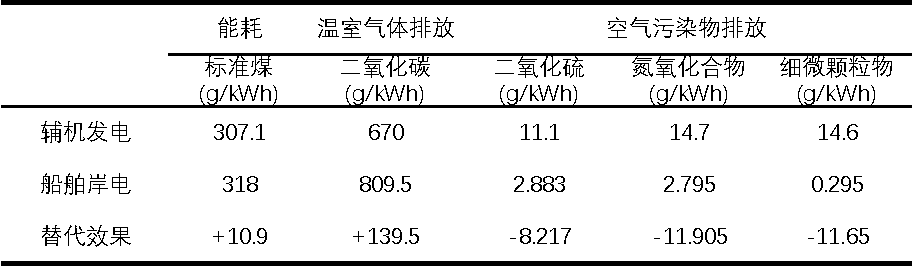
\includegraphics{岸电替代效益.pdf} 
	\end{tabular}
	}
\end{table}





\section{船岸连接系统研究现状}

\zhlipsum[5]

\subsection{国外应用状况}
\zhlipsum[6]
\subsection{国内应用状况}
\zhlipsum[7]
\section{论文研究内容及工作}
\zhlipsum[8]
